\documentclass[12pt,a4paper]{article}
\usepackage[utf8]{inputenc}
\usepackage[brazil]{babel}
\usepackage[T1]{fontenc}
\usepackage[pdftex]{graphicx}
\usepackage[protrusion=true,expansion=true]{microtype}
\usepackage{ae,aecompl}
\usepackage{multirow}
\usepackage{tabularx}
\usepackage{setspace}
\usepackage{textcomp}
\usepackage{bold-extra}
\usepackage{times}
\usepackage{amssymb,amsmath}
\usepackage{sbc-template}
\usepackage{hyperref}
\usepackage{tikz}
\usepackage{booktabs}
\usepackage{placeins}
\usepackage{float}
\usepackage[alf]{abntex2cite}
\bibliographystyle{abnt-alf}
\usepackage{newfloat}

\usepackage{fancyhdr}
\pagestyle{fancy}
\fancyhf{}
\renewcommand{\headrulewidth}{0pt}
\fancyfoot[R]{\thepage}

\sloppy

% wireframe https://www.fluidui.com/editor/live/

\title{Doutor Pecúlio}

\author{Carlos A. O. de Souza Junior\inst{1}
	\and Lucas J. C. Lorenzetti\inst{1} 
	\and Paulo R. Urio\inst{1}}

\address{Departamento de Ciência da Computação (DECOMP) \\
Universidade Estadual do Centro-Oeste (UNICENTRO)\\
Rua Camargo Varela de Sá, 3 -- CEP 85.040-080\\
Guarapuava -- PR -- Brasil -- Telefone: (42) 3629-8100\\
  \email{carlos\_bertojr@hotmail.com, goodlucas@gmail.com, paulo@bk.ru}
}

\hypersetup{
    bookmarks=true,         % show bookmarks bar?
    unicode=false,          % non-Latin characters in Acrobat’s bookmarks
    pdftoolbar=true,        % show Acrobat’s toolbar?
    pdfmenubar=true,        % show Acrobat’s menu?
    pdffitwindow=false,     % window fit to page when opened
    pdfstartview={FitH},    % fits the width of the page to the window
    pdftitle={Doutor Pecúlio},    % title
    pdfauthor={Paulo Urio},     % author
    pdfsubject={IHC},   % subject of the document
    pdfcreator={Paulo Urio},   % creator of the document
    pdfproducer={Paulo Urio}, % producer of the document
    pdfkeywords={android} {ihc} {doutor} {peculio}, % list of keywords
    pdfnewwindow=true,      % links in new window
    colorlinks=true,       % false: boxed links; true: colored links
    linkcolor=black,          % color of internal links
    citecolor=black,        % color of links to bibliography
    filecolor=magenta,      % color of file links
    urlcolor=black           % color of external links
}

\begin{document}

\maketitle
\thispagestyle{fancy}

% Resumo e Abstract

\begin{resumo} 
Neste trabalho foi investigada a elaboração de um projeto preliminar
de uma aplicação interativa de uma assistente pessoal inteligente para
dispositivos móveis, chamado Doutor Pecúlio.  Foram elaborados 
cenários, casos de uso, protótipos com a análise de requisitos
baseada no conhecimento adquirido durante a disciplina de 
interação humano-computador.   

  \item[\hskip\labelsep\bfseries\itshape Palavras-chave.]\itshape{
  engenharia de software; ihc; android; assistente pessoal inteligente.}
  
\end{resumo}

\begin{abstract}
In this study, it was surveyed the project's prospect of an 
intelligent personal assistant to mobile devices, named Doutor Pecúlio.
In order to probe requirements, it were elaborated scenarios, use cases and 
engineering prototypes based on the acquired
knowledge during human-computer interaction classes.

  \item[\hskip\labelsep\bfseries\itshape Palavras-chave.]\itshape{
  software engineering; hci; android; intelligent personal assistant.}
 
\end{abstract}
 % resumo.tex 

%%%%%%%%%%%%%%%%%%%%%%%%%%%%%%%%%%%%%%%%%%%%%%%%%%%%%%%%%%%%%%%%%%%%%%%%
\section{Introdução}

% Em algum momento da introduçào me baseei nisso
% http://people.csail.mit.edu/pcm/tempISWC/workshops/SERES2010/seres10_submission_2.pdf

Somos a sociedade da informação, termo utilizado por
\citeonline{beniger1986control} para referir-se à 
sociedade moderna e seu gradual desejo de controle e consumo da 
informação, desejo este que motivou o
desenvolvimento rápido de tecnologias para o \textit{feedback} automático
em processos industriais, logo no início do período industrial.

Em discussões sobre a sociedade moderna baseadas na dialética do antigo e do novo,
do continuado e do descontinuado, termos como 
capitalismo digital \cite{citeulike:8018090} e
capitalismo virtual \cite{VirtualCapitalism} mostram claramente como
os sistemas computacionais tornaram-se o foco no desenvolvimento tecnológico,
refletindo na criação de uma nova rede cultural e social generalizada, com 
alcance mundial, impactando em uma economia capitalista globalizada.

\citeonline{DBLP:journals/corr/abs-1111-6849} indicam que a geração
de informação cresce exponencialmente.  Como resultado, as pessoas
se veem sobrecarregadas com o volume de informações publicadas em uma
pletora de novos livros e páginas na \textit{internet}, entre outros.  Além disso,
avanços tecnológicos reduziram formidavelmente as barreiras na publicação
e distribuição de informação, através de meios eletrônicos, aumentando a 
dimensão da quantidade de publicações produzidas \cite{rao2008application}.

Na tentativa de amenizar problema do sobrecarregamento de informações e
tentar converter todas as fontes de informação disponíveis em dados úteis,
surgiu o assistente pessoal inteligente (IPA, do inglês \textit{Intelligent
Personal Assistant}) como uma solução factível para auxiliar os usuários
em diferentes domínios de aplicações.

\subsection{Assistente pessoal inteligente}

%{\color{red}
%• Uma descrição sucinta sobre o que você entende por Assistente Pessoal Inteligente 
%para Dispositivos Móveis de forma a definir o escopo de seu projeto. }

Um assistente pessoal inteligente é um agente de \textit{software}
que pode realizar tarefas e serviços para um indivíduo, baseado na
entrada do usuário, como a localização atual e a habilidade para
acessar informações de uma variedade de informações na \textit{internet}, como
condições atuais do clima, do tráfego, notícias, ações, agenda do
usuário e preços de varejo, entre outros \cite{kaschek2007intelligent}.
Exemplos de tais sistemas incluem Google Now \cite{GoogleNow} e 
Siri \cite{Siri}.   Segundo \citeonline{garridoadding}, estes agentes devem 
ser capazes de comunicar, cooperar, discutir com pessoas e também 
guiá-las.

A tecnologia por trás dos assistentes pessoais inteligentes envolve a integração
de dispositivos móveis com \textit{Application Programming Interfaces} (APIs)
públicas,
popularizadas com a proliferação de aplicativos móveis.  
Assistentes inteligentes autônomos são projetados para realizar tarefas
específicas de modo simples através de instruções dadas pelo usuário,
como comandos de voz, redirecionando ações à outros agentes inteligentes,
especializados em realizar tarefas específicas.

Nosso trabalho é voltado ao desenvolvimento da prévia de um agente 
inteligente, especializado em consultar preços de objetos em lojas virtuais
e próximas da localização atual do usuário.

\subsection{Doutor Pecúlio}

Doutor Pecúlio é o nome dado ao aplicativo resultante deste trabalho, o qual
tem o objetivo de agilizar o processo do usuário em consultar preços.
Para interagir, o usuário deve tirar uma foto de um item, que pode ser
por exemplo, a capa de um livro, o código de barras ou o seu código
QR (do inglês, \textit{Quick Response code}).  Em todos os casos, 
necessita-se que o aplicativo
tenha acesso à uma câmera.   O aplicativo é voltado para funcionar com
livros, CDs, DVDs, Blu-ray, mídias para PCs e mídas para consoles de 
\textit{videogame}.

Para uma consulta, precisa-se apenas tirar uma foto da capa do objeto com o 
\textit{smartphone}, ativando a função de câmera.  O usuário pode acessar a
câmera externamente ao programa ou através do menu principal do Doutor Pecúlio.
Com a câmera ativa, é necessário que o usuário alinhe a câmera com o objeto
em uma perspectiva aproximadamente perpendicular.  Após tirar a foto, o 
usuário verifica se a foto ficou boa o suficiente para identificar qual é o
objeto e então inicia a busca.   Para iniciar a busca, existem duas situações.
Se o usuário iniciou a câmera fora do aplicativo, ele deve escolher a opção
de compartilhar a imagem com o Doutor Pecúlio. Porém, se o usuário iniciou
a câmera através do menu do aplicativo, uma opção de confirmar, ou utilizar, a
foto deve ser selecionada.  O aplicativo irá procurar o objeto na 
\textit{internet}, através de uma conexão \textit{Wi-Fi}, onde a consulta
deve ter uma duração aproximada de dois a três segundos antes que os 
resultados comecem a ser mostrados.

Uma vez que uma consulta é realizada com sucesso, o usuário terá acesso
a comentários de avaliações feitos por outros usuários, em \textit{sites} como 
Amazon e Submarino.   Os resultados são ordenados em ordem crescente, sendo
o critério principal o preço do produto e, o secundário, a distância do local, caso o 
resultado seja de uma loja próxima.    Para resultados de lojas locais, 
também são apresentadas direções para chegar e números de telefone, sempre
que possível.

\subsection{Motivação}

Atualmente
existem vários aplicativos móveis que possibilitam a busca de um 
item para consulta e comparação com outras lojas.  Entretanto, muitos necessitam
da entrada manual do usuário, como por exemplo para livros, pode ser
necessário a entrada do identificador ISBN, o autor, o título e
frequentemente detalhes como a
edição do livro que deseja-se consultar.

Com o grande esforço presente na área de pesquisa de visão computacional
relacionados à Recuperação de Imagens Baseada em Conteúdo (CBIR,
do inglês \textit{Content-Based Image Retrieval}) e
Recuperação e Indexação de Imagens Baseada em Conceitos Implícitos (ICIIR,
do inglês, \textit{Implicit Concept-Based Image Indexing and Retrieval}), 
já é possível realizar buscas rápidas por imagens semelhantes em bancos de 
dados grandes, como discutido em \citeonline{jsrgensen2003image},
\citeonline{1265007}, \citeonline{Datta:2008:IRI:1348246.1348248}
e \citeonline{Rui199939}.
\citeonline{Petrakis1993504} discutem os requisitos de \textit{design} e
implementação de um banco de dados de imagens de um sistema que suporta
o armazenamento e recuperação de imagens pelo conteúdo presente nas imagens.

Através destes estudos, acreditamos que seja possível a elaboração de um 
agente inteligente rápido e eficiente, que atenda o usuário de forma 
natural, adequado aos conceitos apresentados por \citeonline{kaschek2007intelligent}, 
sem a necessidade de entrada
manual da descrição do objeto para realizar consultas, almejando ser confortável
e satisfatório ao usuário.

\subsection{Público-alvo}

O usuário que deverá se sentir satisfeito com a usabilidade do aplicativo
é aquele que possui um \textit{smartphone} moderno, com integração à câmera
e conexão \textit{Wi-Fi}.   Imagina-se que este usuário utilizará o
aplicativo em situações corriqueiras, onde o agente causará pouco impacto
na necessidade de atenção ao usuário para sua operação.

% %%
%
%  Atenção: desperdiçando uma referencia passada pela professora:
%   \cite{Rocha}
% %%
  
 % introducao.tex

\FloatBarrier
%%%%%%%%%%%%%%%%%%%%%%%%%%%%%%%%%%%%%%%%%%%%%%%%%%%%%%%%%%%%%%%%%%%%%%%%
\section{Metas de usabilidade e experiência do usuário}

%{\color{red}
%• Um plano de avaliação da interface, deverá ser feita quanto a usabilidade, 
%comunicabilidade e acessibilidade.}

As tecnologias de informação e comunicação oferecem as maneiras
mais eficientes de manipular informações em suas mais variadas formas.
\citeonline{Barbosa} focam em sistemas computacionais interativos,
que fazem cada vez mais parte do cotidiano de todos os usuários.
Em termos de \textit{design} de sistemas móveis, deve-se dar ênfase 
no usuário.  Segundo \citeonline{love2005understanding}, primeiramente,
o \textit{designer} do sistema deve compreender, do início, o que os
usuários vão querer utilizar em um dispositivo móvel, ou seja, quais 
tarefas ele irá realizar enquanto estiver utilizando o sistema.  Em
segundo lugar, quais características do usuário podem afetar
significativamente a usabilidade no sistema, como idade e deficiências
físicas, como por exemplo, cegueira.   Em terceiro lugar, uma vez que o \textit{designer}
tenha levado em consideração as necessidades do usuário, no próximo estágio
deve ser desenvolvido um sistema que adeque-se aos
requisitos identificados na primeira fase.  Então o \textit{designer}
deve testar o sistema para avaliar se o sistema atende às necessidades e
se a utilização é satisfatória.  Com base no \textit{feedback} recebido
durante a avaliação, o \textit{designer} deve produzir uma versão a
atualizada.

Outra característica deve ser levada em conta por ter um grande impacto,
é o contexto de uso, ou seja, em quais ambientes os usuários estarão
ao utilizar o sistema, que afetam na usabilidade, como habilidade, 
eficiência e satisfação ao utilizar.

\subsection{Metas de usabilidade}

%{\color{red}
%• Uma lista com as metas de usabilidade e experiência do usuário a serem atingidas pela 
%aplicação. }

% Um agradecimento ao autor original
% http://www.csl.mtu.edu/cs5760/www/Lectures/CurrentLectures/Usability%20and%20Suite%20Consistency.htm
% :P

\citeonline{rogers2011interaction} sugerem seis metas de usabilidade:
eficácia, eficiência, utilidade, facilidade de aprendizado, capacidade
de memorização e segurança.
Eficácia e utilidade referem-se à funcionalidade do aplicativo.
A eficácia é uma medida geral de como o sistema executa, já a utilidade, é
uma medida das funcionalidades implementadas corretamente e a abrangência
delas.  A eficiência refere-se ao tempo necessário para
utilizar a \textit{interface} e a probabilidade de cometer erros iteragindo
com o sistema.  \textit{Designers} são encorajados a criar 
\textit{interfaces} familiares e naturais, com foco na facilidade de
aprendizado e memorização, ou seja, que possam ser aprendidas
sem a necessidade da leitura de um manual.   No contexto de desenvolvimento
móvel, pouco se discute sobre segurança como uma meta principal de 
usabilidade, pois está mais associada com a garantia de que o usuário
não possa por o sistema em condições periosas do que a segurança como 
consistência de dados.

Como metas pragmáticas de usabilidade para o aplicativo móvel Doutor Pecúlio,
planejamos dar foco em:

\begin{description}
    \item[Aprendizado:] o usuário geralmente não tem tempo e dificilmente
        irá procurar o manual de um aplicativo, o que implica em ter 
        uma \textit{interface} com curva de aprendizagem tênue;
    \item[eficiência:] o usuário não planeja gastar muito tempo
        realizando uma tarefa complexa, portanto, deve ser mantido o
        foco em funcionalidades simples e que possam ser efetuadas
        rapidamente; e
    \item[ergonomia:] as telas dos dispositivos são pequenas, para que o 
        usuário consiga manipular utilizando apenas uma mão, por isso deve
        ser fácil de navegar.
\end{description}

\subsection{Experiência do usuário}

\citeonline{rogers2011interaction} identificam que os objetivos em uma
\textit{interface} gráfica são focados na usabilidade e funcionalidade.
Eles sugerem como metas para experiência a satisfação, agradabilidade,
diversão, entretenimento, prestativo, motivador, estético, motiva
criatividade, recompensador e emocionalmente gratificante.

Para o aplicativo Doutor Pecúlio, selecionamos cinco metas:

\begin{description}
    \item[Prestativo:] o aplicativo deve ter como objetivo ser útil ao 
        usuário em tarefas corriqueiras;
    \item[motivador:] o usuário deve se interessar para utilizar;
    \item[recompensador:] a recompensa irá certificar que o usuário 
        continuará utilizando, após uma interação bem sucedida ele saberá
        que a qualquer momento poderá interagir novamente; e
    \item[agradabilidade:] a taxa de erros de consulta deve ser muito 
        baixa para evitar que o usuário se fruste.
\end{description}
 % metasusabilidaide.tex

\FloatBarrier
%%%%%%%%%%%%%%%%%%%%%%%%%%%%%%%%%%%%%%%%%%%%%%%%%%%%%%%%%%%%%%%%%%%%%%%%
\section{Cenários}

%{\color{red}
%• Uma lista de cenários para os quais se imagina que a aplicação poderá ser aplicada, 
%detalhando 2 cenários principais. }

Um cenário é uma narrativa, a qual descreve todas as interações do usuário
com o sistema durante uma atividade.
Neste trabalho, o objetivo dos cenários é auxiliar a análise de
requisitos funcionais e operacionais do sistema.  Cada cenário descreve como um
sistema deve ser utilizado em um contexto de uma atividade em um prazo de 
tempo definido, sendo que as sub-seções \ref{cenario1} e \ref{cenario2}
descrevem cenários mais detalhados, enquanto que a sub-seção 
\ref{cenario3} descreve um
cenário razoavelmente a alto nível, focando mais em ações feitas ao invés
de operações realizadas a partir de cada ação.

\subsection{Cenário 1} \label{cenario1}

Cenário: Uma tentativa bem sucedida de busca de um produto a partir da
foto da câmera interna do \emph{smartphone}, a qual é utilizada para
tirar uma foto da capa de um livro de interesse do usuário.  O dispositivo
já está conectado à uma rede WiFi.

\begin{enumerate}
\item O usuário inicia a função de câmera;
\item A capa do livro é posicionada de forma aproximadamente ortogonal;
\item O usuário tira uma foto da capa do livro;
\item A foto recém realizada é mostrada ao usuário;
\item O usuário seleciona a opção ``compartilhar'';
\item A opção ``Doutor Pecúlio'' aparece nas opções de compartilhamento,
    a qual é escolhida pelo usuário;
\item O aplicativo ``Doutor Pecúlio'' é iniciado em uma tela onde a foto
    é mostrada escurecida em segundo plano e em primeiro plano é mostrada uma
    mensagem informando que a busca está em andamento;
\item Internamente, como já há conexão estabelecida com a \emph{internet}, o
    algoritmo responsável pelo processamento da imagem é iniciado para identificar
    se a foto é uma capa ou um código de barras ou QR.  O algoritmo identifica que 
    é uma capa e então um segundo algoritmo é executado para criar uma
    identificação única (\emph{hash}) da imagem.   O identificador único é
    utilizado para realizar uma consulta em um servidor dedicado ao aplicativo,
    o qual irá retornar possíveis resultados.  Neste caso, apenas um resultado
    foi encontrado os resultados para aquele título é retornado ao aplicativo.
\item Em aproximadamente três segundos os resultados do livro começam 
    aparecer em uma tela onde mostra a capa \emph{online} do livro e
    resultados encontrados.  Ao lado da capa, o título encontrado é apresentado,
    e logo abaixo a avaliação dos usuários é pela quantidade de estrelas.
    Os resultados são divididos em lojas virtuais
    e lojas locais.  As lojas locais são organizadas em ordem crescente de
    distância e preço, mostradas na tela do usuário.   O usuário pode acessar
    todos os resultados \emph{online} a partir de uma opção mostrada depois
    do título e antes dos resultados locais.    
\end{enumerate}

\subsection{Cenário 2} \label{cenario2}


Cenário: Uma tentativa mal sucedida de busca de um produto a partir da
foto da câmera interna do \emph{smartphone}, a qual é utilizada para
tirar uma foto do código de barras de um DVD de interesse do usuário.  O dispositivo
já está conectado à uma rede WiFi.

\begin{enumerate}
\item O usuário inicia a função de câmera;
\item O código de barras é posicionado de forma aproximadamente ortogonal;
\item O usuário tira uma foto;
\item A foto recém realizada é mostrada ao usuário;
\item O usuário seleciona a opção ``compartilhar'';
\item A opção ``Doutor Pecúlio'' aparece nas opções de compartilhamento,
    a qual é escolhida pelo usuário;
\item O aplicativo ``Doutor Pecúlio'' é iniciado em uma tela onde a foto
    é mostrada escurecida em segundo plano e em primeiro plano é mostrada uma
    mensagem informando que a busca está em andamento;
\item Internamente, como já há conexão estabelecida com a \emph{internet}, o
    algoritmo responsável pelo processamento da imagem é iniciado para identificar
    se a foto é uma capa ou um código de barras ou QR.  O algoritmo identifica que 
    é um código de barras e então um segundo algoritmo é executado para ler o
    código de barras da imagem.   O código de barras é
    utilizado para realizar uma consulta em um servidor dedicado ao aplicativo,
    o qual irá retornar os resultados.  Porém, este DVD ainda não está disponível
    pelas APIs.  O servidor retorna um erro; e
\item Em aproximadamente três segundos a mensagem de erro é mostrada com a
    foto em segundo plano e em primeiro plano é mostrada uma mensagem mostrando
    que o item não foi encontrado.  O usuário tem a opção de poder realizar 
    uma novo foto ou cancelar a operação de busca.
\end{enumerate}

\subsection{Cenário 3} \label{cenario3}

Cenário: Acesso à uma busca já realizada anteriormente.  O dispositivo
não precisa estar conectado à WiFi.

\begin{enumerate}
\item O usuário inicia o aplicativo ``Doutor Pecúlio'';
\item A tela de consultas já realizada é mostrada ao usuário.  Os
    resultados bem sucedidos são mostrados de forma agrupada por tipo 
    de produto consultado, como Livro, DVD e Jogos;
\item O usuário seleciona um resultado de uma busca anterior; e
\item Os mesmos resultados utilizados na busca anterior são mostrados,
    e uma opção de atualizar os resultados é mostrada para que ele possa
    buscar por novos preços e disponibilidade na localidade atual do
    usuário.
\end{enumerate}
 % cenarios.tex

\FloatBarrier
%%%%%%%%%%%%%%%%%%%%%%%%%%%%%%%%%%%%%%%%%%%%%%%%%%%%%%%%%%%%%%%%%%%%%%%%
\section{Personas}

%{\color{red} Texto introdutório para as personas.}

Uma persona, conceito introduzido por \citeonline{cooper2004inmates}, define o 
arquétipo de um usuário de um sistema, um exemplo de um tipo potencial
de pessoa que pode interagir o sistema.  A ideia de uma persona é que
para projetar um \emph{software} efetivo, é necessário que este o seja
projetado para um tipo específico de pessoa.  As personas devem 
representar pessoas fictícias que são baseadas no conhecimento de
pessoas reais.

Nesta seção são descritas três personas.  Foi explorado o foco em pessoas
as quais irão utilizar o aplicativo em situações cotidianas, onde o usuário
pode possivelmente utilizar o aplicativo em paralelo com outras atividades
não relacionadas ao aplicativo.

%\subsection{Persona 1}  \label{sec:persona1}

%%%%%%%%%%%%%%%%%%%%%%%%%%%%% PERSONA %%%%%%%%%%%%%%%%%%%%%%%%%%%%%%%%%%%
\par \noindent
\begin{table}[!ht] 
    \begin{tabularx}{\textwidth}{c}
        \toprule
    \end{tabularx}
    
    \begin{tabularx}{\textwidth}{p{.17\textwidth}p{.5\textwidth}
                                 p{.12\textwidth}p{.101\textwidth}}
        \textbf{Nome:} & Eduardo H. de Mello
        & \textbf{Idade:} & 24 anos \\
    \midrule
    \end{tabularx}
    
    \hspace*{1cm}Eduardo é um rapaz recém formado em Arquitetura e Urbanismo que está de 
mudança para Curitiba, onde foi aprovado no programa de Mestrado da UFPR.
Eduardo necessita comparar preços de livros que possuem poucos exemplares na biblioteca para auxilio durante o mestrado..

\hspace*{1cm}Como planeja realizar compras na cidade de Curitiba -- PR, 
torna-se inexequível a procura do melhor preço em todas as lojas factíveis. 
Não obstante, deseja obter os produtos com os melhores preços, fato que
implica na necessidade de analisar valores em lojas locais e virtuais.
Discretamente, vai à biblioteca s e tira fotos de um
livro de  seu interesse.
Devido as condições da biblioteca,
localiza o código QR do livro.
Ao tirar uma foto do código QR, se estiver conectado à \textit{internet},
em apenas três segundos já deve começar a obter respostas da consulta
para o produto.

\hspace*{1cm}Com os resultados recém consultados, conseguirá analisar os melhores
preços e ler avaliações dos produtos em que teve interesse.  Desta forma, 
poderá saber o local do melhor preço.

\hspace*{1cm}A expectativa é que os preços dos produtos estejam certos, pois isto pode 
fazer com que alguns vendedores das lojas da sua localidade melhorem os preços
em geral, evitando preços muito aquém da média. No decorrer da avalição, como não possui bagagem informativa
sobre as características de eletrodomésticos, além do fato de 
precisar de alguns, a qualificação dos produtos avaliados por outros usuários
como ele, o influenciam na compra de um ou outro determinado produto dentre os
ofertados.
    
    \begin{tabularx}{\textwidth}{c}
        \bottomrule
    \end{tabularx}
    
    \caption{ \label{Persona1} Persona 1}
\end{table}
%%%%%%%%%%%%%%%%%%%%%%%%%%%%% PERSONA %%%%%%%%%%%%%%%%%%%%%%%%%%%%%%%%%%%

%\FloatBarrier
%\subsection{Persona 2}  \label{sec:persona2}
%%%%%%%%%%%%%%%%%%%%%%%%%%%%% PERSONA %%%%%%%%%%%%%%%%%%%%%%%%%%%%%%%%%%%
\par \noindent
\begin{table}[ht]
    \begin{tabularx}{\textwidth}{c}
        \toprule
    \end{tabularx}
    
    \begin{tabularx}{\textwidth}{p{.17\textwidth}p{.5\textwidth}
                                 p{.12\textwidth}p{.101\textwidth}}
        \textbf{Nome:} & Clotilde Van Halen 
        & \textbf{Idade:} & 43 anos \\
    \midrule
    \end{tabularx}
    
    \hspace*{1cm} Clotilde é uma mulher bem sucedida, chefe de família, 
    presidente do grupo de leitura do bairro e gerente geral de uma 
    agência bancária.  Precisou absorver o conhecimento de operação
    de sistemas computacionais desde que começou a trabalhar banco.
    Clotilde, formada em Ciências Econômicas, também passou a ter interesse 
    por tecnologia para pode acompanhar as constantes mudanças que ocorrem 
    no mercado.

    \hspace*{1cm} Ela deseja comprar um \textit DVD do Justin Bieber para sua filha,
    Kimberly, como presente de aniversário de 17 anos.  Clotilde está
    feliz, pois sua filha acabou de ser aprovada no vestibular de Direito na UNIFACIL
    e deseja recompensar sua filha com um presente surpresa.  
    
    \hspace*{1cm} Como a janela de almoço é de apenas uma hora, em horário comercial, 
    deseja localizar rapidamente onde deve comprar um DVD do Justin igual o da filha de  sua 
    colega, Priscila.  Priscila recomenda a Clotilde, a utilização do aplicativo
    Doutor Pecúlio, para que possa descobrir facilmente os locais de venda
    do DVD.   Ao instalar o aplicativo, Clotilde tira uma foto
    do DVD  da filha de  Priscila.
    Desta forma, poderá decidir se vale a pena comprar em uma loja próxima
    ao banco, ou se vale a pena efetuar o pedido via
    \textit{internet}.

\hspace*{1cm}Ao final, aproveita para qualificar o produto escolhido conforme avaliação feita após a consulta 
feita pelo aplicativo. 
    
    \begin{tabularx}{\textwidth}{c}
        \bottomrule
    \end{tabularx}
    
    \caption{ \label{Persona2} Persona 2}
\end{table}
%%%%%%%%%%%%%%%%%%%%%%%%%%%%% PERSONA %%%%%%%%%%%%%%%%%%%%%%%%%%%%%%%%%%%

\FloatBarrier
%\subsection{Persona 3}  \label{sec:persona3}
%%%%%%%%%%%%%%%%%%%%%%%%%%%%% PERSONA %%%%%%%%%%%%%%%%%%%%%%%%%%%%%%%%%%%
\par \noindent
\begin{table}[ht]
    \begin{tabularx}{\textwidth}{c}
        \toprule
    \end{tabularx}
    
    \begin{tabularx}{\textwidth}{p{.17\textwidth}p{.5\textwidth}
                                 p{.12\textwidth}p{.101\textwidth}}
        \textbf{Nome:} & Sirlei da Silva
        & \textbf{Idade:} & 57 anos \\
    \midrule
    \end{tabularx}
    
    \hspace*{1cm} Sirlei é um aposentado que recentemente criou o hábito de ir
    à locadora ver as novidades do cinema. Para não se perder na  megalópoles com seus 
    colegas, utiliza um \textit{smartphone} como GPS (do inglês,
    \textit{Global Positioning System}), porém, o utiliza com óbice,
    não obstante, sempre concretiza as tarefas.

    \hspace*{1cm} Deseja tirar a foto das capas dos filmes para saber qual 
    a média dos preços dos mesmo e saber aproximadamente quando deve  
    recomendar a compra de um filme para alguem ou não. Sirlei incomoda-se de ter que consultar o dono da locadora
    constantemente, pois é uma tarefa extenuante. 
    
    \hspace*{1cm} Deseja que, no fim das contas, possa acessar o registro 
    de todas as consultas feitas enquanto analisava os carros no pátio, 
    no decorrer de cada foto tirada.

    \hspace*{1cm} o caso deste tipo de produto, os anúncios costumam ser 
    temporais e  sempre existem qualificações para os filmes.

    \begin{tabularx}{\textwidth}{c}
        \bottomrule
    \end{tabularx}
    
    \caption{ \label{Persona3} Persona 3}
\end{table}
%%%%%%%%%%%%%%%%%%%%%%%%%%%%% PERSONA %%%%%%%%%%%%%%%%%%%%%%%%%%%%%%%%%%%
 % personas.tex

%%%%%%%%%%%%%%%%%%%%%%%%%%%%%%%%%%%%%%%%%%%%%%%%%%%%%%%%%%%%%%%%%%%%%%%%
\section{Casos de uso}

%{\color{red}
%• Uma lista de casos de uso, detalhando de 2 casos de uso principais. }

%{\color{red}
%• Uma lista de casos de uso essenciais, detalhando de 2 casos de uso essenciais 
%principais. }

Foram considerados quatro casos de uso.  A figura \ref{fig:casos} mostra os
casos de uso de um usuário interagindo com o aplicativo Doutor Pecúlio.
Três casos de uso são possibilidades de busca pela foto da capa, 
código de barras e código QR, respectivamente.   O último caso de uso é
a visualização do histórico de buscas realizadas anteriormente.

\begin{figure}[h]
    \centering
    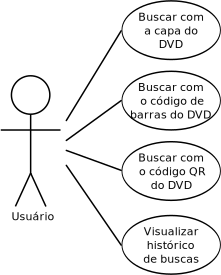
\includegraphics[scale=1]{casos/caso1}
    \caption{ \label{fig:casos} Casos de uso de um usuário interagindo com
        o aplicativo Doutor Pecúlio. }
\end{figure}
 % casosdeuso.tex

\FloatBarrier
%%%%%%%%%%%%%%%%%%%%%%%%%%%%%%%%%%%%%%%%%%%%%%%%%%%%%%%%%%%%%%%%%%%%%%%%
\section{Requisitos do sistema}

A partir dos cenários e casos de uso foram identificados quatro
requisitos funcionais e três requisitos não funcionais.
Os requisitos funcionais são:

\begin{itemize}
\item Integração com as câmeras internas do \emph{smartphone};
\item integração com as APIs de compartilhamento de multimídia;
\item integração com a API GeoIP; e
\item integração com os serviços de lojas virtuais (Amazon.com, Livraria
    Saraiva, Livrarias Curitiba, Livraria Chain, Submarino.com.br).
\end{itemize}

Os requisitos não funcionais são:
\begin{itemize}
\item Acesso à \emph{internet};
\item visualização do histórico de buscas; e
\item acesso ao catálogo de lojas próximas, com base nos resultados
    da API GeoIP.
\end{itemize}

\subsection{Requisitos no modelo de Volere}

%{\color{red}
%• Um conjunto de especificação dos requisitos usando a template do sistema Volere. }

Volere, criado por \citeonline{Robertson:1999:MRP:312381}, é uma coleção de recursos
para levantamento de requisitos, voltada para ajudar a descobrir, compreender,
escrever e comunicar requisitos \cite{VolereOverview}.
Através de modelos flexíveis, o objetivo é melhorar a consistência da estimativa de
tempo, de controle de riscos, monitoramento e reutilização de dados 
analisados.  Foram preenchidos sete requisitos utilizando o modelo de Volere 
disponível \emph{online}\footnote{Disponível em:
<http://www.volere.co.uk/languages.htm>. Acesso em: 11 jun. 2013.}, 
os quais podem ser vistos nas 
tabelas \ref{Volere1}, \ref{Volere2}, \ref{Volere3}, \ref{Volere4},
\ref{Volere5}, \ref{Volere6} e \ref{Volere7}.  Cada requisito contém vários
campos.  Na primeira linha o número do requisito, o tipo de requisito, se este 
é um (1) requisito funcional ou (2) requisito não funcional, e a lista de
casos de uso relacionados.   As três linhas seguintes reportam a
descrição, o nome do requisito, a razão, o motivo de este ser alavancado 
como um requisito e a origem, o nome do autor responsável por propor
o requisito.  Na quinta linha, o critério de ajuste é uma medida que tem
por objetivo propor uma solução para verificar se esta é apropriada às exigências
do requisito.  A satisfação é a quantificação em uma escala de satisfação do 
cliente em relação ao requisito.  Neste trabalho não foram utilizadas escalas
de satisfação, porém os campos foram mantidos para cumprir o modelo.  A sétima
linha lista as dependências para o requisito e a lista de requisitos que são
conflitantes.  As duas últimas linhas reportam os materiais de apoio factíveis
e o histórico de alterações do requisito.


%%%%%%%%%%%%%%%%%%%%%%%%%%%%%%%%%%%%%%%%%%%%%%%%%%%%%%%%%%%%%%%%%%%%%%%%%%
%%%%%%%%%%%%%%%%%%%%%%%%%%%%% TEMPLATE VOLERE %%%%%%%%%%%%%%%%%%%%%%%%%%%%
\par \noindent
\begin{table}[h]
    \begin{tabularx}{\textwidth}{
        p{\dimexpr.18\linewidth-2\tabcolsep-1.3333\arrayrulewidth}
        p{\dimexpr.1\linewidth-2\tabcolsep-1.3333\arrayrulewidth}
        p{\dimexpr.24\linewidth-2\tabcolsep-1.3333\arrayrulewidth}
        p{\dimexpr.14\linewidth-2\tabcolsep-1.3333\arrayrulewidth}
        p{\dimexpr.255\linewidth-2\tabcolsep-1.3333\arrayrulewidth}
        p{\dimexpr.1\linewidth-2\tabcolsep-1.3333\arrayrulewidth}
    }
    \toprule
        \textbf{Requisito \#:}          & 1 
        & \textbf{Tipo de requisito:}   & 1
        & \textbf{Evento/PUC/BUC:}      & 1, 2 \\
    \midrule
    \end{tabularx}
    \vspace{5pt}
    \begin{tabularx}{\textwidth}{p{.12\textwidth}  p{.83\textwidth}}
        \textbf{Descrição:} &
        Integração com as câmeras internas do \emph{smartphone}.
    \end{tabularx}
    
    \vspace{5pt}
    \begin{tabularx}{\textwidth}{p{.12\textwidth}  p{.83\textwidth}}
        \textbf{Razão:} &
        Utilizar as imagens geradas pela câmera como entrada para a 
        busca pelo produto no \emph{software}.
    \end{tabularx}
    
    \vspace{5pt}
    \begin{tabularx}{\textwidth}{p{.12\textwidth} p{.83\textwidth}}
        \textbf{Origem:} &
        Lucas.
    \end{tabularx}
    
    \vspace{5pt}
    \begin{tabularx}{\textwidth}{p{.23\textwidth} p{.72\textwidth}}
        \textbf{Critério de ajuste:} &
        A integração decorre no sentido de que o \emph{software} deve 
        ser capaz de captar as imagens da câmera do usuário quando 
        eles tiram uma foto, independente se é utilizando o sistema 
        para tirar foto ou o próprio \emph{software} de fotos do 
        \emph{smartphone}. 
    \end{tabularx}
    
    \vspace{5pt}
    \begin{tabularx}{\textwidth}{p{.26\textwidth}p{.248\textwidth}
                                 p{.28\textwidth}p{.110\textwidth}}
        \textbf{Satisfação do cliente:} & -- & 
        \textbf{Insatisfação do cliente:} & --
    \end{tabularx}
    
    \vspace{5pt}
    \begin{tabularx}{\textwidth}{p{.17\textwidth}p{.5\textwidth}
                                 p{.12\textwidth}p{.101\textwidth}}
        \textbf{Dependências:} & Depende do acesso ao módulo da 
            câmera via API do \emph{android}.
        & \textbf{Conflitos:} & -- \\
    \end{tabularx}
    
    \vspace{5pt}
    \begin{tabularx}{\textwidth}{p{.235\textwidth} p{.715\textwidth}}
        \textbf{Materiais de apoio:} &
        Documentação da porção do módulo da câmera interna, encontrado
        na documentação para desenvolvedor do \emph{android}.
    \end{tabularx}
    
    \vspace{5pt}
    \begin{tabularx}{\textwidth}{p{.1\textwidth} p{.85\textwidth}}
        \textbf{História:} &
        Criado em 12 de Junho de 2012. \\
    \end{tabularx}
    
    \begin{tabularx}{\textwidth}{c}
        \bottomrule
    \end{tabularx}
    
    \caption{ \label{Volere1} Requisito no modelo de Volere. }
\end{table}
%%%%%%%%%%%%%%%%%%%%%%%%%%%%%%%%%%%%%%%%%%%%%%%%%%%%%%%%%%%%%%%%%%%%%%%%%%



%%%%%%%%%%%%%%%%%%%%%%%%%%%%%%%%%%%%%%%%%%%%%%%%%%%%%%%%%%%%%%%%%%%%%%%%%%
%%%%%%%%%%%%%%%%%%%%%%%%%%%%% TEMPLATE VOLERE %%%%%%%%%%%%%%%%%%%%%%%%%%%%
\par \noindent
\begin{table}[h]
    \begin{tabularx}{\textwidth}{
        p{\dimexpr.18\linewidth-2\tabcolsep-1.3333\arrayrulewidth}
        p{\dimexpr.1\linewidth-2\tabcolsep-1.3333\arrayrulewidth}
        p{\dimexpr.24\linewidth-2\tabcolsep-1.3333\arrayrulewidth}
        p{\dimexpr.14\linewidth-2\tabcolsep-1.3333\arrayrulewidth}
        p{\dimexpr.255\linewidth-2\tabcolsep-1.3333\arrayrulewidth}
        p{\dimexpr.1\linewidth-2\tabcolsep-1.3333\arrayrulewidth}
    }
    \toprule
        \textbf{Requisito \#:}          & 2
        & \textbf{Tipo de requisito:}   & 1
        & \textbf{Evento/PUC/BUC:}      & 1, 2 \\
    \midrule
    \end{tabularx}
    \vspace{5pt}
    \begin{tabularx}{\textwidth}{p{.12\textwidth}  p{.83\textwidth}}
        \textbf{Descrição:} &
        Integração com as APIs de compartilhamento de multimídia.
    \end{tabularx}
    
    \vspace{5pt}
    \begin{tabularx}{\textwidth}{p{.12\textwidth}  p{.83\textwidth}}
        \textbf{Razão:} &
        Para poder usar o aplicativo após fotos tirada pelo aplicativo
        externo de fotos do \emph{smartphone}.
    \end{tabularx}
    
    \vspace{5pt}
    \begin{tabularx}{\textwidth}{p{.12\textwidth} p{.83\textwidth}}
        \textbf{Origem:} &
        Paulo.
    \end{tabularx}
    
    \vspace{5pt}
    \begin{tabularx}{\textwidth}{p{.23\textwidth} p{.72\textwidth}}
        \textbf{Critério de ajuste:} &
        Deve-se desenvolver, de acordo com o as resoluções provenientes 
        da API do sistema operacional a inserção da opção 
        Doutor Pecúlio no menu de aplicativos de compartilhamento,
        o qual direcione a foto ao Doutor Pecúlio diretamente para a
        fase de busca do produto.
    \end{tabularx}
    
    \vspace{5pt}
    \begin{tabularx}{\textwidth}{p{.26\textwidth}p{.248\textwidth}
                                 p{.28\textwidth}p{.110\textwidth}}
        \textbf{Satisfação do cliente:} & -- & 
        \textbf{Insatisfação do cliente:} & --
    \end{tabularx}
    
    \vspace{5pt}
    \begin{tabularx}{\textwidth}{p{.17\textwidth}p{.5\textwidth}
                                 p{.12\textwidth}p{.101\textwidth}}
        \textbf{Dependências:} & Depende de como a API do \emph{android}
        é implementada.
        & \textbf{Conflitos:} & -- \\
    \end{tabularx}
    
    \vspace{5pt}
    \begin{tabularx}{\textwidth}{p{.235\textwidth} p{.715\textwidth}}
        \textbf{Materiais de apoio:} &
       Documentação da API do módulo da lista de opções de 
       compartilhamento do \emph{android}.
    \end{tabularx}
    
    \vspace{5pt}
    \begin{tabularx}{\textwidth}{p{.1\textwidth} p{.85\textwidth}}
        \textbf{História:} &
        Criado em 12 de Junho de 2012. \\
    \end{tabularx}
    
    \begin{tabularx}{\textwidth}{c}
        \bottomrule
    \end{tabularx}
    
    \caption{ \label{Volere2} Requisito no modelo de Volere. }
\end{table}
%%%%%%%%%%%%%%%%%%%%%%%%%%%%%%%%%%%%%%%%%%%%%%%%%%%%%%%%%%%%%%%%%%%%%%%%%%


%%%%%%%%%%%%%%%%%%%%%%%%%%%%%%%%%%%%%%%%%%%%%%%%%%%%%%%%%%%%%%%%%%%%%%%%%%
%%%%%%%%%%%%%%%%%%%%%%%%%%%%% TEMPLATE VOLERE %%%%%%%%%%%%%%%%%%%%%%%%%%%%
\par \noindent
\begin{table}[h]
    \begin{tabularx}{\textwidth}{
        p{\dimexpr.18\linewidth-2\tabcolsep-1.3333\arrayrulewidth}
        p{\dimexpr.1\linewidth-2\tabcolsep-1.3333\arrayrulewidth}
        p{\dimexpr.24\linewidth-2\tabcolsep-1.3333\arrayrulewidth}
        p{\dimexpr.14\linewidth-2\tabcolsep-1.3333\arrayrulewidth}
        p{\dimexpr.255\linewidth-2\tabcolsep-1.3333\arrayrulewidth}
        p{\dimexpr.1\linewidth-2\tabcolsep-1.3333\arrayrulewidth}
    }
    \toprule
        \textbf{Requisito \#:}          & 3
        & \textbf{Tipo de requisito:}   & 1
        & \textbf{Evento/PUC/BUC:}      & 1 \\
    \midrule
    \end{tabularx}
    \vspace{5pt}
    \begin{tabularx}{\textwidth}{p{.12\textwidth}  p{.83\textwidth}}
        \textbf{Descrição:} &
        Integração com a API GeoIP.
    \end{tabularx}
    
    \vspace{5pt}
    \begin{tabularx}{\textwidth}{p{.12\textwidth}  p{.83\textwidth}}
        \textbf{Razão:} &
        Obter informação da localização atual do usuário,
        utilizando a API GeoIP.
    \end{tabularx}
    
    \vspace{5pt}
    \begin{tabularx}{\textwidth}{p{.12\textwidth} p{.83\textwidth}}
        \textbf{Origem:} &
        Lucas.
    \end{tabularx}
    
    \vspace{5pt}
    \begin{tabularx}{\textwidth}{p{.23\textwidth} p{.72\textwidth}}
        \textbf{Critério de ajuste:} &
        O aplicativo deve ter acesso a informação do identificador
        IP da conexão atual do \emph{smartphone} para poder,
        através do GeoIP, descobrir a localização atual e então
        utilizar como critério de busca de catálogos de lojas
        próximas.
    \end{tabularx}
    
    \vspace{5pt}
    \begin{tabularx}{\textwidth}{p{.26\textwidth}p{.248\textwidth}
                                 p{.28\textwidth}p{.110\textwidth}}
        \textbf{Satisfação do cliente:} & -- & 
        \textbf{Insatisfação do cliente:} & --
    \end{tabularx}
    
    \vspace{5pt}
    \begin{tabularx}{\textwidth}{p{.17\textwidth}p{.5\textwidth}
                                 p{.12\textwidth}p{.101\textwidth}}
        \textbf{Dependências:} & Conseguir adquirir o endereço de IP da
        conexão atual.
        & \textbf{Conflitos:} & -- \\
    \end{tabularx}
    
    \vspace{5pt}
    \begin{tabularx}{\textwidth}{p{.235\textwidth} p{.715\textwidth}}
        \textbf{Materiais de apoio:} &
       Documentação da API do GeoIP.
    \end{tabularx}
    
    \vspace{5pt}
    \begin{tabularx}{\textwidth}{p{.1\textwidth} p{.85\textwidth}}
        \textbf{História:} &
        Criado em 12 de Junho de 2012. \\
    \end{tabularx}
    
    \begin{tabularx}{\textwidth}{c}
        \bottomrule
    \end{tabularx}
    
    \caption{ \label{Volere3} Requisito no modelo de Volere. }
\end{table}
%%%%%%%%%%%%%%%%%%%%%%%%%%%%%%%%%%%%%%%%%%%%%%%%%%%%%%%%%%%%%%%%%%%%%%%%%%


%%%%%%%%%%%%%%%%%%%%%%%%%%%%%%%%%%%%%%%%%%%%%%%%%%%%%%%%%%%%%%%%%%%%%%%%%%
%%%%%%%%%%%%%%%%%%%%%%%%%%%%% TEMPLATE VOLERE %%%%%%%%%%%%%%%%%%%%%%%%%%%%
\par \noindent
\begin{table}[h]
    \begin{tabularx}{\textwidth}{
        p{\dimexpr.18\linewidth-2\tabcolsep-1.3333\arrayrulewidth}
        p{\dimexpr.1\linewidth-2\tabcolsep-1.3333\arrayrulewidth}
        p{\dimexpr.24\linewidth-2\tabcolsep-1.3333\arrayrulewidth}
        p{\dimexpr.14\linewidth-2\tabcolsep-1.3333\arrayrulewidth}
        p{\dimexpr.255\linewidth-2\tabcolsep-1.3333\arrayrulewidth}
        p{\dimexpr.1\linewidth-2\tabcolsep-1.3333\arrayrulewidth}
    }
    \toprule
        \textbf{Requisito \#:}          & 4
        & \textbf{Tipo de requisito:}   & 1
        & \textbf{Evento/PUC/BUC:}      & 1 \\
    \midrule
    \end{tabularx}
    \vspace{5pt}
    \begin{tabularx}{\textwidth}{p{.12\textwidth}  p{.83\textwidth}}
        \textbf{Descrição:} &
        Integração com os serviços de lojas virtuais (Amazon.com, 
        Livraria Saraiva, Livrarias Curitiba, Livraria Chain, 
        Submarino.com.br).
    \end{tabularx}
    
    \vspace{5pt}
    \begin{tabularx}{\textwidth}{p{.12\textwidth}  p{.83\textwidth}}
        \textbf{Razão:} &
        Poder consultar preços dos livros, CD's, DVD's, BD's, etc.
    \end{tabularx}
    
    \vspace{5pt}
    \begin{tabularx}{\textwidth}{p{.12\textwidth} p{.83\textwidth}}
        \textbf{Origem:} &
        Carlos.
    \end{tabularx}
    
    \vspace{5pt}
    \begin{tabularx}{\textwidth}{p{.23\textwidth} p{.72\textwidth}}
        \textbf{Critério de ajuste:} &
        Todas as livrarias que tenham disponibilizados seus 
        catálogos na \emph{internet}.
    \end{tabularx}
    
    \vspace{5pt}
    \begin{tabularx}{\textwidth}{p{.26\textwidth}p{.248\textwidth}
                                 p{.28\textwidth}p{.110\textwidth}}
        \textbf{Satisfação do cliente:} & -- & 
        \textbf{Insatisfação do cliente:} & --
    \end{tabularx}
    
    \vspace{5pt}
    \begin{tabularx}{\textwidth}{p{.17\textwidth}p{.5\textwidth}
                                 p{.12\textwidth}p{.101\textwidth}}
        \textbf{Dependências:} & Disponibilidade dos dados das 
        livrarias.  Necessário o título, desejável o preço.
        & \textbf{Conflitos:} & -- \\
    \end{tabularx}
    
    \vspace{5pt}
    \begin{tabularx}{\textwidth}{p{.235\textwidth} p{.715\textwidth}}
        \textbf{Materiais de apoio:} &
       Fornecimento da documentação necessária para integração, 
       de preferência uma API global entre várias lojas, como a
       API do eBay.
    \end{tabularx}
    
    \vspace{5pt}
    \begin{tabularx}{\textwidth}{p{.1\textwidth} p{.85\textwidth}}
        \textbf{História:} &
        Criado em 12 de Junho de 2012. \\
    \end{tabularx}
    
    \begin{tabularx}{\textwidth}{c}
        \bottomrule
    \end{tabularx}
    
    \caption{ \label{Volere4} Requisito no modelo de Volere. }
\end{table}
%%%%%%%%%%%%%%%%%%%%%%%%%%%%%%%%%%%%%%%%%%%%%%%%%%%%%%%%%%%%%%%%%%%%%%%%%%


%%%%%%%%%%%%%%%%%%%%%%%%%%%%%%%%%%%%%%%%%%%%%%%%%%%%%%%%%%%%%%%%%%%%%%%%%%
%%%%%%%%%%%%%%%%%%%%%%%%%%%%% TEMPLATE VOLERE %%%%%%%%%%%%%%%%%%%%%%%%%%%%
\par \noindent
\begin{table}[h]
    \begin{tabularx}{\textwidth}{
        p{\dimexpr.18\linewidth-2\tabcolsep-1.3333\arrayrulewidth}
        p{\dimexpr.1\linewidth-2\tabcolsep-1.3333\arrayrulewidth}
        p{\dimexpr.24\linewidth-2\tabcolsep-1.3333\arrayrulewidth}
        p{\dimexpr.14\linewidth-2\tabcolsep-1.3333\arrayrulewidth}
        p{\dimexpr.255\linewidth-2\tabcolsep-1.3333\arrayrulewidth}
        p{\dimexpr.1\linewidth-2\tabcolsep-1.3333\arrayrulewidth}
    }
    \toprule
        \textbf{Requisito \#:}          & 5
        & \textbf{Tipo de requisito:}   & 2
        & \textbf{Evento/PUC/BUC:}      & 1, 2, 3 \\
    \midrule
    \end{tabularx}
    \vspace{5pt}
    \begin{tabularx}{\textwidth}{p{.12\textwidth}  p{.83\textwidth}}
        \textbf{Descrição:} &
        Acesso à \emph{internet}. 
    \end{tabularx}
    
    \vspace{5pt}
    \begin{tabularx}{\textwidth}{p{.12\textwidth}  p{.83\textwidth}}
        \textbf{Razão:} &
        Consulta de preços em lojas virtuais.
    \end{tabularx}
    
    \vspace{5pt}
    \begin{tabularx}{\textwidth}{p{.12\textwidth} p{.83\textwidth}}
        \textbf{Origem:} &
        Carlos.
    \end{tabularx}
    
    \vspace{5pt}
    \begin{tabularx}{\textwidth}{p{.23\textwidth} p{.72\textwidth}}
        \textbf{Critério de ajuste:} &
        O \emph{smartphone} precisa de mecanismos para conectar à
        um meio de acesso à \emph{internet}, como redes ad-hoc,
        WiFi ou 3G.
    \end{tabularx}
    
    \vspace{5pt}
    \begin{tabularx}{\textwidth}{p{.26\textwidth}p{.248\textwidth}
                                 p{.28\textwidth}p{.110\textwidth}}
        \textbf{Satisfação do cliente:} & --& 
        \textbf{Insatisfação do cliente:} & --
    \end{tabularx}
    
    \vspace{5pt}
    \begin{tabularx}{\textwidth}{p{.17\textwidth}p{.5\textwidth}
                                 p{.12\textwidth}p{.101\textwidth}}
        \textbf{Dependências:} & --
        & \textbf{Conflitos:} & -- \\
    \end{tabularx}
    
    \vspace{5pt}
    \begin{tabularx}{\textwidth}{p{.235\textwidth} p{.715\textwidth}}
        \textbf{Materiais de apoio:} &
       --
    \end{tabularx}
    
    \vspace{5pt}
    \begin{tabularx}{\textwidth}{p{.1\textwidth} p{.85\textwidth}}
        \textbf{História:} &
        Criado em 12 de Junho de 2012. \\
    \end{tabularx}
    
    \begin{tabularx}{\textwidth}{c}
        \bottomrule
    \end{tabularx}
    
    \caption{ \label{Volere5} Requisito no modelo de Volere. }
\end{table}
%%%%%%%%%%%%%%%%%%%%%%%%%%%%%%%%%%%%%%%%%%%%%%%%%%%%%%%%%%%%%%%%%%%%%%%%%%


%%%%%%%%%%%%%%%%%%%%%%%%%%%%%%%%%%%%%%%%%%%%%%%%%%%%%%%%%%%%%%%%%%%%%%%%%%
%%%%%%%%%%%%%%%%%%%%%%%%%%%%% TEMPLATE VOLERE %%%%%%%%%%%%%%%%%%%%%%%%%%%%
\par \noindent
\begin{table}[h]
    \begin{tabularx}{\textwidth}{
        p{\dimexpr.18\linewidth-2\tabcolsep-1.3333\arrayrulewidth}
        p{\dimexpr.1\linewidth-2\tabcolsep-1.3333\arrayrulewidth}
        p{\dimexpr.24\linewidth-2\tabcolsep-1.3333\arrayrulewidth}
        p{\dimexpr.14\linewidth-2\tabcolsep-1.3333\arrayrulewidth}
        p{\dimexpr.255\linewidth-2\tabcolsep-1.3333\arrayrulewidth}
        p{\dimexpr.1\linewidth-2\tabcolsep-1.3333\arrayrulewidth}
    }
    \toprule
        \textbf{Requisito \#:}          & 6
        & \textbf{Tipo de requisito:}   & 2
        & \textbf{Evento/PUC/BUC:}      & 3 \\
    \midrule
    \end{tabularx}
    \vspace{5pt}
    \begin{tabularx}{\textwidth}{p{.12\textwidth}  p{.83\textwidth}}
        \textbf{Descrição:} &
        Visualização do histórico de buscas.
    \end{tabularx}
    
    \vspace{5pt}
    \begin{tabularx}{\textwidth}{p{.12\textwidth}  p{.83\textwidth}}
        \textbf{Razão:} &
        Poder rever, resgatar, reavaliar e/ou lembrar o que foi 
        buscado/visualizado com Dr. Pecúlio.
    \end{tabularx}
    
    \vspace{5pt}
    \begin{tabularx}{\textwidth}{p{.12\textwidth} p{.83\textwidth}}
        \textbf{Origem:} &
        Paulo.
    \end{tabularx}
    
    \vspace{5pt}
    \begin{tabularx}{\textwidth}{p{.23\textwidth} p{.72\textwidth}}
        \textbf{Critério de ajuste:} &
        Uma maneira eficiente de guardar o histórico, ou seja, 
        integração com algum tipo de conta na \emph{internet}, o qual
        permita que o usuário possa acessar de outro computador
        e compartilhar em redes sociais.
    \end{tabularx}
    
    \vspace{5pt}
    \begin{tabularx}{\textwidth}{p{.26\textwidth}p{.248\textwidth}
                                 p{.28\textwidth}p{.110\textwidth}}
        \textbf{Satisfação do cliente:} & -- & 
        \textbf{Insatisfação do cliente:} & --
    \end{tabularx}
    
    \vspace{5pt}
    \begin{tabularx}{\textwidth}{p{.17\textwidth}p{.5\textwidth}
                                 p{.12\textwidth}p{.101\textwidth}}
        \textbf{Dependências:} & Conta de usuário e armazenamento 
        do histórico com dados criptografados para a segurança.
        & \textbf{Conflitos:} & -- \\
    \end{tabularx}
    
    \vspace{5pt}
    \begin{tabularx}{\textwidth}{p{.235\textwidth} p{.715\textwidth}}
        \textbf{Materiais de apoio:} &
       --
    \end{tabularx}
    
    \vspace{5pt}
    \begin{tabularx}{\textwidth}{p{.1\textwidth} p{.85\textwidth}}
        \textbf{História:} &
        Criado em 12 de Junho de 2012. \\
    \end{tabularx}
    
    \begin{tabularx}{\textwidth}{c}
        \bottomrule
    \end{tabularx}
    
    \caption{ \label{Volere6} Requisito no modelo de Volere. }
\end{table}
%%%%%%%%%%%%%%%%%%%%%%%%%%%%%%%%%%%%%%%%%%%%%%%%%%%%%%%%%%%%%%%%%%%%%%%%%%

\FloatBarrier

%%%%%%%%%%%%%%%%%%%%%%%%%%%%%%%%%%%%%%%%%%%%%%%%%%%%%%%%%%%%%%%%%%%%%%%%%%
%%%%%%%%%%%%%%%%%%%%%%%%%%%%% TEMPLATE VOLERE %%%%%%%%%%%%%%%%%%%%%%%%%%%%
\par \noindent
\begin{table}[h]
    \begin{tabularx}{\textwidth}{
        p{\dimexpr.18\linewidth-2\tabcolsep-1.3333\arrayrulewidth}
        p{\dimexpr.1\linewidth-2\tabcolsep-1.3333\arrayrulewidth}
        p{\dimexpr.24\linewidth-2\tabcolsep-1.3333\arrayrulewidth}
        p{\dimexpr.14\linewidth-2\tabcolsep-1.3333\arrayrulewidth}
        p{\dimexpr.255\linewidth-2\tabcolsep-1.3333\arrayrulewidth}
        p{\dimexpr.1\linewidth-2\tabcolsep-1.3333\arrayrulewidth}
    }
    \toprule
        \textbf{Requisito \#:}          & 7
        & \textbf{Tipo de requisito:}   & 2
        & \textbf{Evento/PUC/BUC:}      & 1, 2, 3 \\
    \midrule
    \end{tabularx}
    \vspace{5pt}
    \begin{tabularx}{\textwidth}{p{.12\textwidth}  p{.83\textwidth}}
        \textbf{Descrição:} &
        Acesso ao catálogo das lojas próximas, com base nos resultados 
        da API GeoIP.
    \end{tabularx}
    
    \vspace{5pt}
    \begin{tabularx}{\textwidth}{p{.12\textwidth}  p{.83\textwidth}}
        \textbf{Razão:} &
         Para poder informar preços das lojas mais próximas.
    \end{tabularx}
    
    \vspace{5pt}
    \begin{tabularx}{\textwidth}{p{.12\textwidth} p{.83\textwidth}}
        \textbf{Origem:} &
        Paulo.
    \end{tabularx}
    
    \vspace{5pt}
    \begin{tabularx}{\textwidth}{p{.23\textwidth} p{.72\textwidth}}
        \textbf{Critério de ajuste:} &
        A loja deve existir de maneira \emph{online} e ter informações 
        disponíveis.
    \end{tabularx}
    
    \vspace{5pt}
    \begin{tabularx}{\textwidth}{p{.26\textwidth}p{.248\textwidth}
                                 p{.28\textwidth}p{.110\textwidth}}
        \textbf{Satisfação do cliente:} & -- & 
        \textbf{Insatisfação do cliente:} & --
    \end{tabularx}
    
    \vspace{5pt}
    \begin{tabularx}{\textwidth}{p{.17\textwidth}p{.5\textwidth}
                                 p{.12\textwidth}p{.101\textwidth}}
        \textbf{Dependências:} & Conexão com \emph{internet} e
        a loja ser disponibilizada \emph{online}.
        & \textbf{Conflitos:} &--\\
    \end{tabularx}
    
    \vspace{5pt}
    \begin{tabularx}{\textwidth}{p{.235\textwidth} p{.715\textwidth}}
        \textbf{Materiais de apoio:} &
       --
    \end{tabularx}
    
    \vspace{5pt}
    \begin{tabularx}{\textwidth}{p{.1\textwidth} p{.85\textwidth}}
        \textbf{História:} &
        Criado em 12 de Junho de 2012. \\
    \end{tabularx}
    
    \begin{tabularx}{\textwidth}{c}
        \bottomrule
    \end{tabularx}
    
    \caption{ \label{Volere7} Requisito no modelo de Volere. }
\end{table}
%%%%%%%%%%%%%%%%%%%%%%%%%%%%%%%%%%%%%%%%%%%%%%%%%%%%%%%%%%%%%%%%%%%%%%%%%%

 % requisitos.tex

%\FloatBarrier
%%%%%%%%%%%%%%%%%%%%%%%%%%%%%%%%%%%%%%%%%%%%%%%%%%%%%%%%%%%%%%%%%%%%%%%%
\section{Protótipos}
%{\color{red}
%• Os protótipos de baixo nível (em papel) usado para definir o projeto da aplicação, caso 
%tenham sido usados. }

%{\color{red}
%• Um protótipo em wireframe do sistema, com as justificativas (baseadas nos princípios 
%de usabilidade, conceitos de design e nas metas estabelecidas no item 1) para a 
%escolha e alocação de cada elemento de interface. }

%\subsection{Protótipo de baixo nível}  {\color{red} OK -- não foi utilizado }
%\subsection{Protótipo de alto nível}

Para a criação dos protótipos foi utilizado o \emph{software} de 
prototipação Fluid UI criado por Kearney e Hannigan em 2010,
disponível \emph{online}\footnote{Disponível em:
<https://www.fluidui.com/>. Acesso em: 28 abr. 2013.}.
A figura \ref{fig:TelaHistorico} mostra os \emph{mockups} para a tela de
consultas já realizadas, do lado esquerdo, e a tela de uma
consulta em andamento, do lado direito.  A figura
 \ref{fig:TelaHarryPotter} mostra os \emph{mockups} para as telas de resultado.
 Ao lado esquerdo a tela de uma busca bem sucedida, com a foto
 da capa encontrada \emph{online}, o título e a avaliação da
 comunidade, com os preços logo em seguida.  Ao lado direito
 está a tela de busca mal sucedida, onde uma mensagem de erro é mostrada
 solicitando o usuário a tirar uma nova foto.  No caso de uma busca mal
 sucedida, o usuário pode ter tirado uma foto de forma inadequada,
 como mostrada na figura, onde a foto está borrada pelo movimento
 praticado pelo usuário durante a captação da imagem.

Os protótipos desenvolvidos utilizam listas, botões, diálogos e imagens.
Um botão consiste de um texto que comunica claramente a ação que será
tomada quando o usuário o toca.   Neste \emph{design} foi utilizado apenas
um botão, com bordas para facilitar a identificação do artefato como
botão.  
Um diálogo é um pedido ao usuário para tomar uma decisão de controle ou
oferecer informações adicionais necessárias para que a aplicação continue
sua tarefa.  Tais pedidos podem ser desde decisões de OK/Cancelar para
leiautes mais complexos que pedem ao usuário ajustes de configurações
adicionais. Por fim,
uma lista apresenta múltiplos itens em várias linhas dispostas em um
leiaute vertical.  Listas são utilizadas para seleção de dados ou para
a navegação de dados sendo visualizados.

%{\color{red} justificar cada elemento da interface }
\begin{figure}[ht]
        \begin{minipage}{.5\textwidth}
            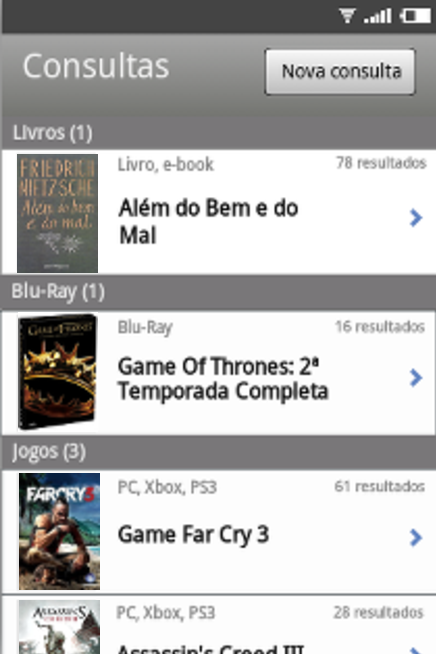
\includegraphics[scale=1]{tela/TelaHistorico}
        \end{minipage}
        \begin{minipage}{.5\textwidth}
            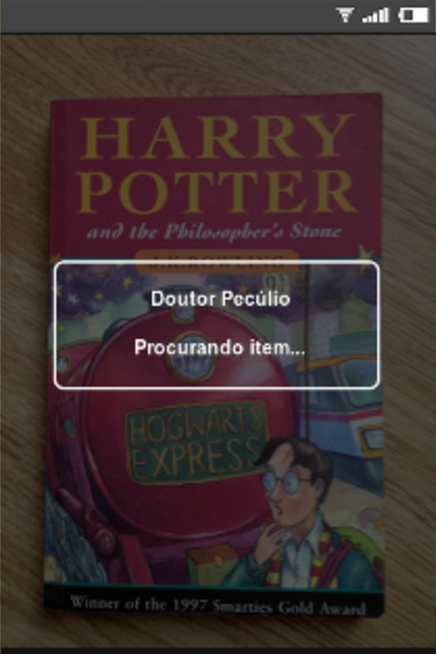
\includegraphics[scale=1]{tela/TelaBuscando}
        \end{minipage}
        \caption{ \label{fig:TelaHistorico} \textit{Mockups} para telas de 
            histórico de consultas e uma consulta em andamento. }

        \begin{minipage}{.5\textwidth}
            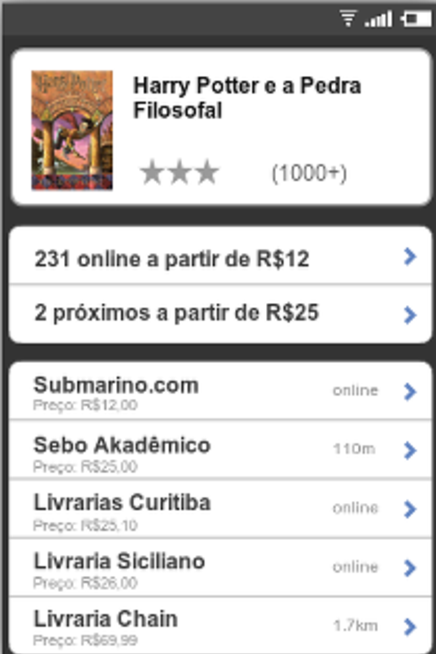
\includegraphics[scale=1]{tela/Tela}
        \end{minipage}
        \begin{minipage}{.5\textwidth}
            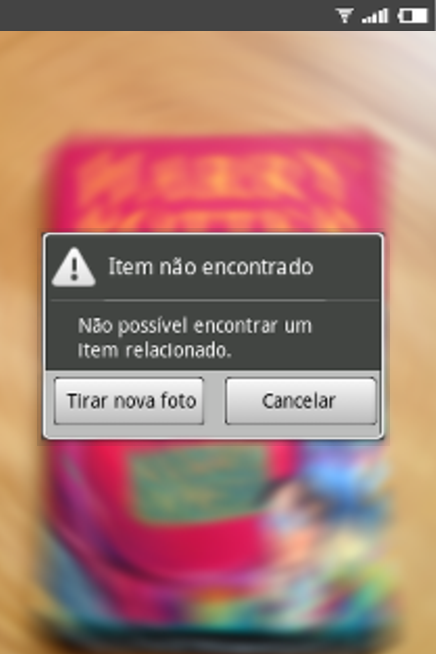
\includegraphics[scale=1]{tela/TelaErro}
        \end{minipage}
        \caption{ \label{fig:TelaHarryPotter} \textit{Mockups} para telas de 
            resultados bem e mal sucedidos. }
\end{figure}
 % prototipos.tex

\FloatBarrier
%%%%%%%%%%%%%%%%%%%%%%%%%%%%%%%%%%%%%%%%%%%%%%%%%%%%%%%%%%%%%%%%%%%%%%%%
\section{Avaliação da interface}

Percurso cognitivo (do inglês, \emph{Cognitive Walkthrough}), criado por
\citeonline{Wharton:1994:CWM:189200.189214} é um método de inspeção de
usabilidade utilizado para identificar problemas em sistemas interativos.
A avaliação heurística (do inglês, \emph{Heuristic Evaluation}), criado
por \citeonline{Nielsen:1990:HEU:97243.97281}, é um método de inspeção
de usabilidade utilizado para identificar problemas no
\emph{design} da interface de usuário.
O Método de Inspeção Semiótica (MIS) e o Método de Avaliação de 
Comunicabilidade (MAC), da Engenharia Semiótica, tem como
objetivo analisar a qualidade da comunicação entre
\emph{designer} e usuário através da interface de sistemas interativos
\cite{deSouza:2006:SIM:1298023.1298044}.

Neste trabalho o protótipo desenvolvido foi avaliado utilizando o 
percurso cognitivo, a avaliação heurística, MIS e MAC, para avaliar
a comunicabilidade e a usabilidade.

\subsection{Percurso cognitivo}

Porção do sistema escolhida: Acessar a lista de consultas realizadas.

Passo único: Abrir o aplicativo doutor pecúlio, a lista de consultas recentemente realizada esta 
na pagina inicial do aplicativo.

\begin{itemize}
\item O usuário tentará atingir a meta correta?
    \begin{itemize}
    \item Dada a decomposição de uma tarefa em sub-tarefas, o usuário saberá por onde começar? 
        Saberá qual é o próximo passo? \\
        Não existem sub-tarefas, a única tarefa é abrir o aplicativo.
    \item O que o usuário vai tentar fazer a cada momento?
        Navegar pela lista de consultas tocando na tela e visualizando as ultimas consultas realizadas.
    \end{itemize}
\item O usuário perceberá que a ação correta está disponível na interface?
    \begin{itemize}
        \item Onde está o elemento de interface correspondente ao próximo passo? O usuário pode vê-lo 
            ou sabe onde ele está? \\
        Só existe um paço que é abertura do aplicativo,
    \item Que ações a interface torna disponíveis? \\
       Este passo se torna desnecessário.
    \end{itemize}
\item Uma vez encontrado o elemento de interface, o usuário reconhecerá que ele produzirá o 
efeito desejado?
    \begin{itemize}
        \item O elemento de interface revela seu propósito e comportamento? \\
        Sim uma vez que a lista de consulta está disponibilizada logo no inicio do aplicativo.
    \item O usuário consegue identificar os elementos de interface? \\
      O usuário não enfrenta grandes dificuldades, pois a tarefa é simples.
    \end{itemize}
\item Após a ação correta ser executada, o usuário perceberá que progrediu em direção à solução 
da tarefa?
    \begin{itemize}
        \item Como a interface apresenta o resultado de cada ação? \\
        Nesta ação apenas aparece na tela a lista de consultas passadas. 
    \item O resultado apresentado tem correspondência com o objetivo do usuário? \\
      O protótipo é viável.
    \end{itemize}
\end{itemize}

\subsection{Avaliação heurística}

\par \noindent \textbf{Elemento da interface:} Lista de consultas já realizadas.
\par \noindent \textbf{Localização:} Tela inicial.
\par \noindent \textbf{Heurística violada:} Falta de contraste entre e fundo e cores.
\par \noindent \textbf{Gravidade:} 1 -- cosmético.
\par \noindent \textbf{Recomendação de solução:} Utilizar cores vivas.

\subsection{Método de Inspeção Semiótica (MIS)}

Os mentores deste trabalho, avaliam como é comunicação na porção aonde aparece a o item 
``Procurando...'', encontrado na tela à direita da
figura \ref{fig:TelaHistorico}, o programador quer passar pro usuário que o produto está sendo procurado 
na \emph{internet}, como objetivo da inspeção semiótica é identificar a ruptura na comunicação dos 
elementos de uma interface.

Cenário: Um usuário hipotético, alfabetizado, mas que recém comprou um 
\emph{smartphone} e não tem 
muita perícia com o equipamento, resolve tirar uma foto de um livro e nas opções de 
compartilhar escolhe o aplicativo Doutor Pecúlio, semelhante à 
figura \ref{fig:TelaHistorico} à direita. A mensagem 
do \emph{designer} quando colocou ``procurando item'' e deixou a foto em segundo plano, 
foi com o objetivo de
mostrar que o sistema estava procurando o produto que teve a foto tirada.
 O autores calculam que o tempo necessário para o recebimento
de uma resposta é de até três segundos.
Se o sistema demorar muito, ele pode achar que não conseguiu realizar esta tarefa, que o 
sistema travou, e então, sai do aplicativo e começa todo processo novamente, a ruptura na 
comunicação ocorreu quando o sistema deveria dar um indicativo de que estava trabalhando, 
ou algo do gênero.

\subsection{Método de Avaliação de Comunicabilidade (MAC)}

\par \noindent
\begin{enumerate}
\item Preparação
    \begin{itemize}
    \item Definição dos objetivos da investigação; \\
        Avaliar se o usuário é capaz de visualizar o que já havia consultados.
    \item Escolha dos participantes; \\
        A escolha é o próprio autor da avaliação, Lucas José Campos 
        Lorenzetti.
    \item Elaboração de roteiro de observação do teste; \\
        O roteiro será observando se existem dificuldades do usuário em entender que 
        naquela porção do sistema é que se localizam as suas consultas já realizadas.
    \item Executar teste-piloto; \\
        A tela utilizada foi a tela à esquerda da figura \ref{fig:TelaHistorico}.
    \end{itemize}
\item Aplicação
    \begin{itemize}
    \item Cenário -- Narrativa envolvente na qual haja um personagem com o 
        qual os participantes do teste (usuários) possam identificar:
        \begin{itemize}
        \item Atividade que este personagem deve realizar \\
            Abrir o aplicativo doutor pecúlio e visualizar suas consultas já realizadas.
        \end{itemize}
    \item Entrevista pós-teste -- Impressões gerais do participante:
        \begin{itemize}
        \item Eliminar ambiguidades para a etiquetagem posterior \\
            Aparece a etiqueta \textsc{Socorro!} Se o usuário não consegue realizar a tarefa.
        \end{itemize}
    \end{itemize}
\item Interpretação
    \begin{itemize}
    \item O avaliador deve etiquetar os vídeos da interação;
    \item Etiquetar -- Colocar ``palavras na boca do usuário'' --
        Ex.: ``Cadê?'', ``Desisto'', ``Onde estou?'', ``Vai de outro jeito!'' e etc.
    \item As etiquetas identificam tipos definidos de rupturas na comunicação; \\
        \begin{figure}[h]
            \begin{minipage}{.4\textwidth}
                \hfill
                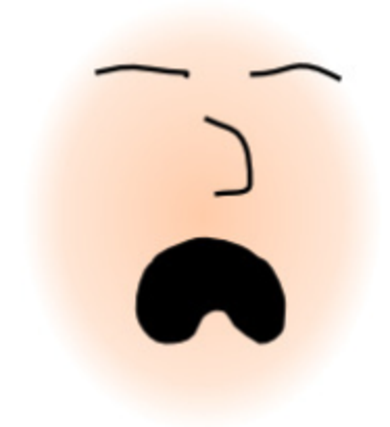
\includegraphics[scale=.5]{LixoSono}
                \vfill
            \end{minipage} 
            \begin{minipage}{.6\textwidth}
                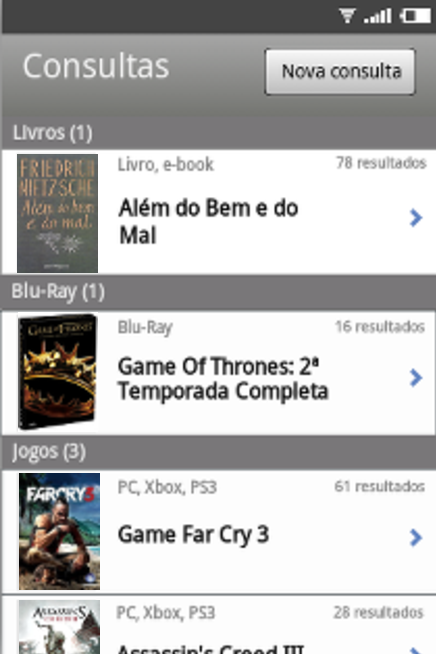
\includegraphics[scale=1]{tela/TelaHistorico}
            \end{minipage}
            \caption{Neste ponto podem surgir rupturas de comunicação.}
        \end{figure}
    \end{itemize}
\item Consolidação dos resultados
    \begin{itemize}
    \item Perguntas-guia:
    \item Qual a frequência das etiquetas por participante, por atividade (do cenário de teste), 
        por elemento da interface ou qualquer outro critério que a equipe de avaliadores 
        considerar relevante?  \\
        Podem haver no ponto inicial aonde o programa não informa
            exatamente que aquelas são as ultimas buscas.
    \item Quais padrões de ocorrência das etiquetas no contexto das atividades entre os 
        participantes?\\
        Uma vez apenas, já que foram feitos um teste piloto.
    \item Os tipos ou sequências de etiquetas podem ser associados a problemas no 
        estabelecimento das metas e submetas de comunicação? \\
        \begin{figure}[h]
            \centering
            
\includegraphics[scale=.5]{LixoMorto}
            \caption{O usuário por ventura desiste da tarefa.}
        \end{figure}
    \end{itemize}
\item Relato dos resultados
    \begin{itemize}
    \item 
        O objetivo era ver se o usuário iria conseguir saber que aquela porção era relativa a suas 
        últimas pesquisas realizadas, e a conclusão preliminar, visualizando o único caminho, após ter 
        sido aberto o \emph{software}, a etiquetagem resultou em ``socorro'' já que a função não estava 
        evidente e pode dizer ``desisto'' quando pode acreditar que não existe aquela porção do 
        sistema, a sugestão de melhoria seria então colocar um texto dizendo ``últimas consultas''
        antes de aparecerem as últimas consultas do usuário.
    \end{itemize}
\end{enumerate}

 % avaliacao.tex

\FloatBarrier
%%%%%%%%%%%%%%%%%%%%%%%%%%%%%%%%%%%%%%%%%%%%%%%%%%%%%%%%%%%%%%%%%%%%%%%%
\section{Considerações finais}
De acordo com a perspectiva de mercado aonde as pessoas cada dia mais tem acesso a 
\emph{smartphones} e a maioria dos \emph{shoppings} tem acesso à rede 
WiFi, além das tecnologias de redes 
móveis e \emph{ad-hoc}, tornam o uso de um aplicativo digital viável, com o crescimento emergente 
do uso de lojas de comercio virtuais por parte de lojas reais, a possibilidade de uso de GeoIP e 
outros métodos de localização, o Dr. Peculio se mostra um sistema viável, com potencial e com 
diferencial no mercado.

O objetivo deste trabalho foi além de mostrar a documentação básica oriunda da 
Engenheira de Software e os requisitos de avaliações por parte da interação 
humano-computador, para que em trabalhos futuros, sirva de referencia para a composição de um 
\emph{software} similar que tome por base esta poderosa ideia.
 % conclusao.tex

\FloatBarrier
%%%%%%%%%%%%%%%%%%%%%%%%%%%%%%%%%%%%%%%%%%%%%%%%%%%%%%%%%%%%%%%%%%%%%%%%
\bibliography{references}

\end{document}
